\chapter{Overview}
In this chapter, we introduce basic information and define essential terminology from~the~field of~bioinformatics. We describe different ways for solving the problem of~gene tree reconciliation with examples of existing software in more details.

\section{Background}
Every organism has its complete set of genetic information encoded in a genome. A~genome consists of~several DNA (deoxyribonucleic acid) molecules and contains all the~information, which are required for~the~organism to~function.

DNA is a long molecule composed of~two complementary strands. Each strand is made up of~four chemical bases: adenine, guanine, cytosine and thymine, and connected to its complementary strand by~pairing rules, where adenine is paired up with~thymine and cytosine is paired up with~guanine. The~sequence of~these bases encodes the~genetic information important for~building and maintaining an~organism. Specific parts of~DNA are called genes.

A gene is a subsequence of~a~DNA strand that contains information for~the~synthesis of~a~specific molecule, usually a~protein. It is a~basic unit of~heredity.

The DNA sequence of a gene can be altered by mutation. It is a process that allows small changes in~the~DNA of~organisms that refers to~differences between individuals within a~population. We will be working with two types of mutations: duplication and gene loss.

Duplication is a~type of~mutation where one or more genes are copied and inserted to~some other position in~the same genome. A~duplicated gene sometimes develops a~new function \cite{doyon}. 

The opposite of~duplication is gene loss (deletion). It~is a~type of~mutation in~which some part of~a~DNA sequence containing a~gene is left~out from~the~genome during DNA replication or it~loses its function. 

Speciation is an~evolutionary process of~in~which a~single population evolves populations into~two distinct species. It can happen for~various reasons, for~example, when a~group separates from~other members of~its species to~a~different geographical area. Members of~a~new group develop their own unique characteristics due to~the~demands of~another environment and this process will differentiate the~new species.

Duplications and speciations result in the~formation of groups of~similar genes, called gene families, from a~single gene. A~gene family consists of~evolutionarily related genes from one or multiple species, which are structurally and usually functionally similar.

Evolutionary relationships formed by~evolutionary events are represented in~a~form of~graph called a~phylogenetic tree, which is a~branching diagram that~shows evolutionary relationships between organisms. A~phylogenetic tree is a~tree~$T$ with nodes~$V(T)$, edges~$E(T)$ and leaves~$L(T)$. It is called weighted when branch length~$w(u, v)$ is defined for~each edge~$(u, v)$.

Phylogenetic trees can be either rooted or unrooted (Fig. \ref{unrooted_rooted}). A~rooted tree is a~phylogenetic tree $T$ where for $(u, v) \in E(T)$: node $u$ is the parent of node $v$, node $v$ is the children of node $u$, $root(T)$ does not have parent and leaves $L(T)$ do not have children. An ancestor of node $v$ is any node of tree $T$ on the path from node $v$ to $root(T)$. Every ancestor have at least one descendant. An descendant of node $v$ is any node of tree $T$ of which $v$ is an ancestor \cite{hasic}. We will denote for $u, v \in V(T)$ that $v<_Tu$ if~$u$ is ancestor of~$v$ and $v$ is descendant of~$u$.

Every rooted tree has a height, which symbolizes the longest path. It is the number of nodes between the $root(T)$ and one of the leaves. 

If a rooted tree is weighted, nodes in the tree have depths. The depth of node $u$, $D(u)$, is the sum of the lengths of all edges between node $u$ and the $root(T)$ of a rooted tree.

For~a~group of~nodes in~a~rooted tree, their~lowest common ancestor~(LCA) is the~farthest node from~the~root that has all nodes in~the~group as~descendants.

An~unrooted tree is a~phylogenetic tree without root. Unrooted tree can be rooted by~placing a~root $r$ on some edge $(u, v)$. The~original edge $(u, v)$ is subdivided into two edges $(u, r)$ and $(r, v)$. If~edge $(u, v)$ is weighted, then $w(u, r) + w(r, v) = w(u, v)$.

A special type of an unrooted tree is a semi-rooted tree, where we presume the new root of an unrooted gene tree $G$ is positioned on edge $(u, v) \in E(G)$ and subtrees are rooted at nodes $u$ and $v$.

\begin{figure}[ht]
	\centering
	\label{unrooted_rooted}
  	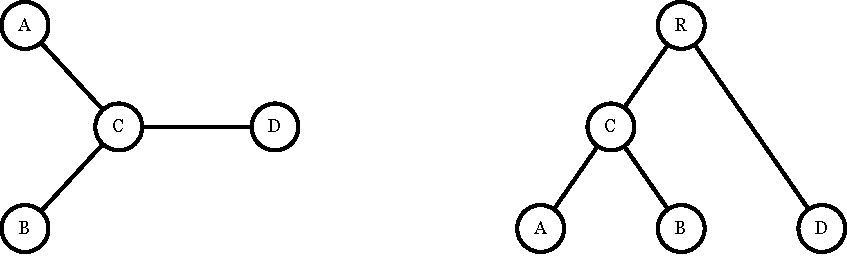
\includegraphics[width=\linewidth]{unrooted_rooted}
  	\caption[Unrooted tree and its~rooted version]{Unrooted tree(left) and its~rooted version (right) tree. We~placed the~root~$R$ on~the~edge~$(C, D)$ replacing it with~two new edges~$(C, R)$ and~$(R, D)$.}
\end{figure}

We will be using two types of phylogenetic trees for showing evolutionary relationships: species trees (to describe the~evolution of~a~set of~species) and gene trees (to describe the~evolution of~a~particular gene).

A~species tree is a~phylogenetic tree $S$ where $L(S)$ represent present-day species and internal nodes from $V(S)$ represent speciation events in~the~history.

A~gene tree is a~phylogenetic tree $G$ where $L(G)$ represent present-day copies of~the~gene and internal nodes from $V(S)$ represent duplication and gene loss events in~the~history.

Phylogenetic trees are reconstructed from a~multiple alignments of~the~DNA sequences of~present-day species by~various methods \cite{felsenstein} to find the~most likely phylogenetic tree to given DNA sequences.

\section{Different approaches to gene tree reconciliation}
Evolutionary history is a possible sequence of~evolutionary events that lead to~observed members of~a~gene family in~present-day species (Fig. \ref{reconciliation}). It illustrates how many duplications and gene losses happened during the~evolution of~one or more genes inside the evolution of~a~group of~species.

The~problem of~gene tree and species tree reconciliation was introduced in~1979 by~Goodman~et~al.~\cite{goodman} as~a~method to~infer the~evolutionary history of~duplications and gene losses in~a~gene family to~decode evolutionary relationships between copies of~a~gene. The goal of~reconciliation consists in~mapping nodes of a gene tree into a species tree and thus inducing the~evolution of~a gene family in~terms of~speciations, duplications and gene losses. An important prerequisite for~reconciliation is to~have a~gene tree without errors as~misplaced leaves can lead to~a different history of~the gene family.

\begin{definition}
A reconciliation between gene tree $G$ and species tree $S$ is mapping $\phi: V(G) \rightarrow V(S)$ such that:
	\begin{enumerate}\itemsep0em
	\item $\forall u \in L(G): \phi(u) = \mu(u)$
	\item $\forall u, v \in V(G)$ such that $v<_Gu$: $\phi(v)<_S\phi(u)$
	\end{enumerate}
	\label{def_reconciliation}
\end{definition}

An example of gene tree reconciliation is shown in Figure \ref{reconciliation}. We are given the gene tree $G$, the species tree $S$ and a leaf mapping $\mu: L(G) \rightarrow L(S)$ that maps each leaf from $G$ to leaf of its species in $S$. We will map internal nodes according to the second condition in Definition \ref{def_reconciliation}. Software.Node $d$ is mapped to node $Y$, because it has $\phi(d)$ and $\phi(c)$ as descendants. It cannot be mapped to node $X$ since node $X$ does not have $\phi(c)$ as descendant thus $\phi(c)<_S\phi(d)$ would not hold. Then node $e$ is mapped above node $Y$ to have $\phi(a)$ and $\phi(d)$ as descendants.

\begin{figure}[ht]
	\centering
	\label{reconciliation}
  	\includegraphics[width=\linewidth]{reconciliation}
  	\caption[Reconciliation and evolutionary history]{Reconciliation and evolutionary history. On~the~left, the~gene tree~$G$ is mapped to~the~species tree~$S$. On~the~right, we~can see the evolutionary history implied by this reconciliation. This~history contains one~duplication $e$, two speciations $Y$ and $X$ and three gene losses (empty circles).}
\end{figure}

The LCA-mapping $\sigma: V(G) \rightarrow V(S)$ maps each node $u \in V(G)$ as low as possible to~the~unique node $\sigma(u) = LCA(\mu(v) | \forall v \in L(G), v<_Gu)$ in $S$. It satisfy both conditions in Definition \ref{def_reconciliation} and minimize the number of duplications and gene losses. This reconciliation can be found in linear time \cite{hasic}.

In this work, we divide approaches to reconciliation into three types: scoring, probabilistic and isometric. Every one of these approaches has its way to compute the gene tree reconciliation. They will be described with presented examples of software that have implemented gene tree reconciliation. 

\subsection{Scoring gene tree reconciliation}
One of the known approaches to find the best reconciliation is to minimize the duplication-loss score, which signifies the sum of duplications and gene losses during the reconciliation. Various software for scoring gene tree reconciliation are known such as TreeBeST, TreeFix, Treerecs or Notung.\\
\textbf{TreeBeST} 

Software TreeBeST \cite{treebest_online} takes a rooted species tree and multiple sequence alignment of gene trees for the gene family as input. It uses a method to merge various input gene trees into one gene tree with a model to penalize duplications and gene losses relative to a known species tree. The method first resolves the topology of a gene tree with five methods: neighbour-joining synonymous distance, non-synonymous distance, p-distance and max-likelihood under the WAG and the HKY model. Then the topology is bootstrapped 100 times. The output of the software is one rooted tree.

The TreeBeST reconciliation method was then compared with PhyML+RAP method, where multiple sequence alignment of gene trees are reconciled to one gene tree without the presence of species tree \cite{treebest}. To evaluate these two methods, authors developed a duplication consistency score represented by \( \frac{intersection}{union} \) of species between left and right branches. Low duplication consistency score means poor topology of the resultant gene tree. PhyML+RAP approach leads to more duplication nodes that TreeBeST and the supplementary duplication nodes made by PhyML+RAP had a low duplication consistency score. Authors found this result unexpected as TreeBeST uses the species tree and tends to produce duplication when the gene tree has extensive extant members on each side of the duplication.\\
\textbf{TreeFix}  

TreeFix \cite{treefix_tutorial} takes a rooted species tree, a maximum likelihood gene tree and a multiple sequence alignment of gene trees for the gene family as input. It infers duplications and gene losses using maximum parsimony reconciliation with a~duplication-loss cost function, which looks for the reconciliation with the~minimum total number of duplications and gene losses. Duplication ($D$) and gene loss ($L$) have their costs ($c_D$ and $c_L$) that are set to one by default and can be changed by the~user. The duplication-loss cost for one reconciliation can be written as: $c_D \cdot D+c_L \cdot L$. 

The main method \cite{treefix} uses a hill-climbing search strategy to find an optimal rooted gene tree with the statistically equivalent likelihood to the given maximum likelihood gene tree and with minimum duplication-loss cost as output. Basics of the method are to compute duplication-loss cost and perform neighbour interchange and subtree prune and regraft on the current optimal gene tree. After finding proposals, it chooses the proposal with the lowest duplication-loss cost and with the statistically equivalent likelihood to the given maximum likelihood gene tree. This process is repeated for a given number of iterations.

Authors compared TreeFix with RAxML, SPIMAP, TreeBeST, Notung and tt using simulated and real datasets of two types of species: 12 Drosophila and 16 fungi \cite{treefix_online}. The software was judged from the point of view of phylogenetic accuracy in 5 categories (topology, branch, orthologs, duplications, losses) and runtime. TreeFix and SPIMAP show the best accuracy in all 5 categories, Notung has slightly worse accuracy in reconstructing the topology of fungi and precision of inferring duplication and gene losses. tt has problems in the same categories as Notung. The worst accuracy demonstrate RAxML and TreeBeST. While TreeFix and SPIMAP have great phylogenetic accuracy their average running time is longer than others. The best runtime has Notung followed by tt and RAxML.\\
\textbf{Treerecs} 

Software Treerecs \cite{treerecs_tutorial} takes a rooted species tree, one or more rooted or unrooted gene trees and a mapping of gene tree leaves to species tree leaves. It provides reconciling gene tree within the associated species tree minimizing the duplication and gene loss score and rooting the gene tree along the way if needed. The output is, depending on the input, one or more rooted gene trees.

The main aim of the authors was to create a more efficient software. They compared Treerecs with EcceTERA, Notung and Ranger-DTL in 3 categories: root (find the root that minimizes duplication-loss score), correction and root+correction (do both previous categories at the same time). In the first category, Treerecs is better than Ranger-DTL and Notung, which shows a large increase in execution time as the number of leaves increases. Treerecs show the best performance in the correction of trees followed by Notung, while Ranger-DTL has big execution time even with a small increase of leaves. The last category is only supported by Treerecs and EcceTERA, where Treerecs has also better performance.\\
\textbf{Notung}  

Notung \cite{notung} takes a rooted species tree, a rooted or unrooted gene tree and the leaf mapping as input. If the gene tree is not rooted, it can be rooted by Notung rooting mode that gives each edge a root score (weighted sum of duplications and gene losses). Apart from a reconciliation of binary trees, Notung can reconcile binary gene trees with non-binary species trees and non-binary gene trees with the binary species tree. The non-binary tree is a tree with at least one polytomy (a node with more than two children). Reconciliation of binary gene trees to non-binary species trees results into binary gene tree.

They use an algorithm, that can distinguish between duplication and deep coalescence (divergence, when the time of separation of two lineages precede the time of speciation) and leads to the smaller total number of duplications and losses than duplication-loss cost function used in reconciliation of two binary trees \cite{vernot}. The duplication-loss cost function is the same as in TreeFix. Reconciliation of non-binary gene tree to binary species tree results into non-binary gene tree. The general approach is to convert the non-binary gene tree to binary gene tree that has minimal duplication-loss score when reconciled with the binary species tree. The resolution is then rearranged back to non-binary gene tree, where all nodes and edges not present in the original gene tree are removed and their assigned duplications and gene losses are reassigned to their polytomy.

\subsection{Probabilistic gene tree reconciliation}
Probabilistic methods have been designed to~increase the~accuracy of~reconciled trees. We~introduce two software tools that use probabilistic methods to~reconcile gene trees: SPIMAP and Phyldog.\\
\textbf{SPIMAP}

SPIMAP software~\cite{spimap_online} takes a rooted species tree and multiple gene sequences of species from the species tree. Normally, the gene sequences are compared and clustered according to their similarity, which results in a set of homologous gene families. Each gene family has its multiple sequence alignment that is reconstructed into gene trees and they are reconciled with the known species tree. Into this classic pipeline, SPIMAP inserts a parameter estimation model using Bayesian approach creating a new phylogenomic pipeline. It learns duplication, gene loss rates during clustering and gene, species substitution rates during the process of alignment. These parameters are then used while building and reconciling the gene tree with the known species tree. The output is a special reconciliation file format that contains gene node ID, species node ID and evolutionary event that occurred on a given node.

The~parameter estimation model \cite{spimap} infers duplication and gene loss rate using the~birth-death process. The birth-death process is a continuous-time process that generates a gene tree according to the~constant birth rate (representing duplication) and death rate (representing gene loss). After running it for a time that represents branch length, all branches that exist at the time are "surviving" and others are "extinct". If a node has no surviving descendants, it is called "doomed". Every branch has its length, which can be written as  \( \frac{substitutions}{site} \) or a product of a duration of time and a substitution rate. The substitution rates signify the number of substitutions per site per unit of time. The model computes gene-specific rate (measures all rate in a tree) for every gene family and species-specific (specifies rate to given branch in the gene tree) rate for every branch.

To determine if the new phylogenomic pipeline improved accuracy, authors compare SPIMAP with PrIME-GSR, SPIDIR, MrBayes, PHYML, BIONJ, RAxML and SYNERGY. They used the same data as TreeFix: 12 Drosophila and 16 fungi. Firstly, they measured the average runtime. The best runtime, under 1 minute, have RAxML, MrBayes, PhyML and BionJ, which was the fastest method. With the same amount of iterations, SPIMAP was quicker than SPIDIR or PrIME-GSR, which was the slowest method. Next, they decided to apply the duplication consistency score (used in TreeBeST) to determine method with better accuracy. The smallest number of duplication with low duplication consistency score have SPIMAP and SYNERGY. The moderate performance shows PrIME-GSR and SPIDIR. Remaining four methods have a similar number of duplication with low duplication consistency score. Lastly, they evaluate phylogenetic accuracy depending on 5 categories (used in TreeFix) for 6 above-mentioned methods (except RAxML and SYNERGY). SPIMAP has higher accuracy in every category. In the category of inferring the topology, PrIME-GSR has slightly worse accuracy while SPIDIR, MrBayes, PHYML, BIONJ shows bad accuracy in the topology of fungi dataset. The accuracy of reconstructed branches is better than the topology in every method, SPIMAP and PrIME-GSR are first two. SPIDIR, MrBayes, PHYML, BIONJ are a little worse at the sensitivity of detection orthologs in fungi dataset. They have the biggest problem with the precision of inferring the duplications in fungi dataset and losses in both datasets. The same problem has also PrIME-GSR, but only in precision of inferring losses.\\
\textbf{PhylDog}

Another software is~PhylDog \cite{phyldog_online} takes multiple gene alignments, a mapping between gene names and species names, and a list of species names as input. The method infers species tree, gene trees, duplication and gene loss rates by maximizing the probability of alignments overall gene families composed from the likelihood of a phylogeny given an alignment and the likelihood of the reconciliation of a gene tree with a species tree according to duplication and gene loss rates. This method uses the birth-death process and is similar to SPIMAP, but they differ in~two aspects. First, while SPIMAP assumes duplication and gene loss rates to~be~constant for~all branches in~the~species tree, PhylDog chooses to~use a~particular pair of~duplication and gene loss rates to~each branch of~the~species tree. Second, SPIMAP requires time-anchored species tree (branch length shows the~amount of~time between two nodes) to compute the~likelihood of~a~gene family. Alternately, PhylDog calculates likelihood from~the~expected numbers of~duplications and gene losses. The output is reconciled gene trees.

PhylDog was compared with TreeBeST and PhyML \cite{phyldog} in terms of the number of duplications and the reconstructed ancestral genome size. PhyML has the biggest number of predicted duplication events, TreeBeST reconciled trees with a much smaller number, but still much higher than PhylDog. The same order of software was also in the number of reconstructed ancestral genome size, where both PhyML and TreeBeST have bigger ancestral genomes that lead to deeper nodes in the species tree.

\subsection{Isometric gene tree reconciliation}
Another variant of reconciliation is isometric gene tree reconciliation, where both species tree $S$ and gene tree $G$ has known branch lengths. These branch lengths are taken into account while mapping a gene tree $G$ to a species tree $S$. The output of isometric reconciliation is reconciled gene tree with preserved evolutionary distances. The branch lengths of phylogenetic tree express estimated time between evolutionary events. The time can signify the actual geological time, amount of evolutionary changes that happened on the edge or expected number of substitution per site between two nodes.

\subsubsection{Exact branch length}

This~problem was introduced and named by~Ma~et~al.~\cite{ma} in~2008 for the first time. They defined isometric reconciliation of rooted species tree and unrooted gene trees, where all input trees have exact branch lengths. The algorithm executes all input gene trees one by one. First of all, it maps all leaves from the gene tree to leaves in the species tree. Then it takes an unmapped node, which has to be connected with at least 2 already mapped nodes, and call function, that map the unmapped node into the species tree and root the gene tree. The presented algorithm had $O(N^2)$ running time, where $N$ stands for the total number of nodes in the gene tree and the species tree. However, their definition of isometric reconciliation has some flaws since it does not preserve all evolutionary distances between nodes as it allows them to develop a reconciliation that does not satisfy any history of evolution.

As a result, Brejová~et~al.~\cite{brejova} later corrected and modified algorithm by~Ma~et~al. to a more efficient algorithm with $O(N \log N)$ running time. Their modify algorithm firstly maps every leaf from gene tree to the species tree. Next, it maps all unmapped nodes to the species tree. After all nodes are correctly mapped, the algorithm roots the gene tree and maps the found root to the species tree. Eventually, it verifies if the reconciled tree is correct due to the definition of isometric reconciliation. They also proposed two extensions of the problem. In the first extension, they considered both input trees (gene tree and species tree) to be unrooted and designed an~algorithm with~$O(N^5 \log N)$ running time. The second extension presents an~algorithm, where both input trees are rooted, but gene tree branch lengths are assumed to be scaled by an unknown scaling factor.

\begin{definition}
An isometric reconciliation between gene tree $G$ and species tree $S$ with exact branch lengths $w$, which are strictly positive, is mapping $\phi: V(G) \rightarrow V(S) \times R$ such that:
	\begin{enumerate}\itemsep0em
	\item $\forall u \in L(G): \phi(u) = [\mu(u), 0]$
	\item $\forall u, v \in V(G)$ such that $v<_Gu$: $\phi(v)<_S\phi(u)$ and $w(u, v) = d(\phi(u), \phi(v))$, where $d$ is the length of path between $u$ and $v$ in reconciled gene tree.
	\end{enumerate}
\end{definition}

\begin{figure}[ht]
	\centering
	\label{isometric_reconciliation}
  	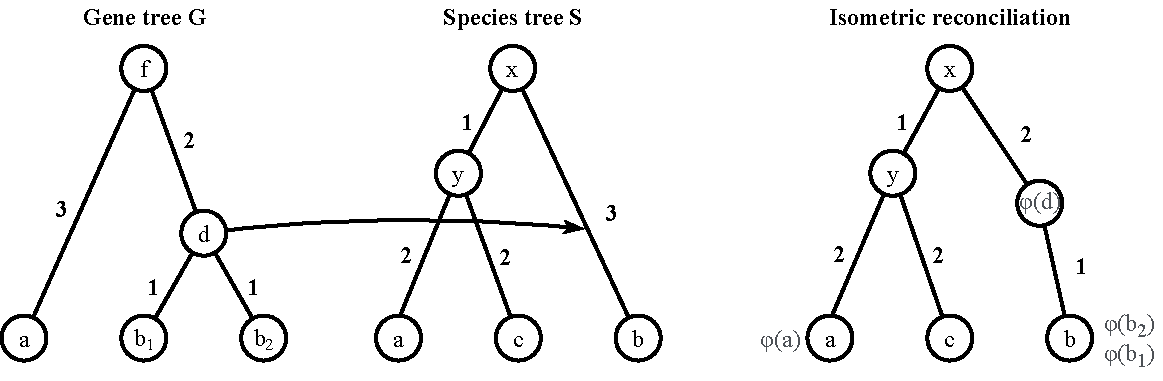
\includegraphics[width=\linewidth]{isometric_reconciliation}
  	\caption[Isometric reconciliation]{Isometric reconciliation. On~the~left is mapping of~the~node~$d$ of~the~gene tree~$G$ to~the~edge~$(x, b)$ of~the~species tree~$S$. The result of~the~isometric reconciliation with~mapped node~$d$ is on~the~right.}
\end{figure}

\subsubsection{Inexact branch lengths} \label{Inexact_branch_lengths}

Input to the above-mentioned algorithms, gene trees and species trees with their branch lengths, are practically estimated from DNA sequences, which were gathered from present-day species \cite{felsenstein}. The branch lengths are computed from observed mutations in collected DNA sequences. However, mutations happen randomly in the evolution and DNA sequences are also random samples from studied present-day species. It means that inferred gene trees and species trees with their branch lengths are estimated with an error.

\begin{figure}[ht]
	\centering
	\label{isometric_reconciliation_inexact}
  	\includegraphics[width=\linewidth]{isometric_reconciliation_inexact}
  	\caption[Isometric reconciliation with inexact branch lengths]{Isometric reconciliation with inexact branch lengths. On the left, we can see an unrooted gene tree G with inexact branch lengths and a rooted species tree S. On the right are two possible solutions with rooting the gene tree on the edge $(u, c)$: the first reconciliation is without duplications and gene losses while the second solution maps gene tree to species tree with two duplications ($u$ and $r$) and four gene losses.}
\end{figure}

To avoid defectiveness and make isometric reconciliation more precise, the isometric reconciliation with inexact branch lengths was introduces by Chládek in \cite{chladek_unpublished} and \cite{chladek_thesis}. They define inexact branch length as an interval, where for every weighted edge stands: $w(u, v) = \langle w(u, v)_{min}, w(u, v)_{max} \rangle$. They present three types of algorithm.\\
\textbf{Linear programming algorithm}

The algorithm is based on linear programming and takes a rooted species tree and a rooted gene tree with inexact branch lengths as an input. They introduce a term of mapping depth, which represents a depth of mapped node $u \in V(G)$ in species tree: $D(\phi(u))$. The solution of isometric reconciliation is to find mapping depths to all nodes from gene tree to species tree. They suggest a set of 5 inequalities that can be solved by a linear program.

The first two inequalities assume that the difference of mapping depths of two nodes, where the one is a parent and the other is his child, has to be between the maximal and minimal length of the edge. The second two inequalities are similar and say that the distance between depths of two neighbouring nodes in species tree must be within the maximal and minimal length of the edge. Last inequality restricts mapping depth of node from gene tree to be same smaller than the depth of its LCA-mapping node in the species tree. The algorithm also defines that leaves from gene tree map to leaves from species tree and the root of the species tree is in depth 0, so every node, which maps above the root has negative depths. 

For $N$ nodes, the algorithm can get to the result in polynomial time. It also works if the gene tree and species tree are non-binary trees. With a few changes in inequalities, the linear program can find reconciliation to semi-rooted and unrooted species and gene trees.\\
\textbf{Two-pass algorithm} \label{two-pass_algorithm}

The two-pass algorithm is faster than the linear programming algorithm. The input for the algorithm is a rooted species tree with exact branch lengths and a rooted gene tree with inexact branch lengths. It consists of two parts: upward and downward sweep. 

The upward sweep goes from the leaves of the gene tree to the root and it computes preliminary interval $\langle x[u]_{min}, x[u]_{max} \rangle$ for each node $u$. The interval is a set of all potential mapping depths values of node $u$ over all reconciliations of a subtree of the gene tree rooted at node $u$ to the species tree. It does not take into account the rest of the gene tree, only the descendants of node $u$. The highest mapping point of node $u$, $x[u]_{min}$, is computed by taking the maximum value of both children highest mapping points subtracted by the longest branch length values. Similarly is calculated the lowest mapping point $x[u]_{max}$, where both children lowest mapping points are subtracted by the shortest branch length values and the minimum of these values is taken. If $x[u]_{min} > x[u]_{max}$, the interval is empty thus for the input is no reconciliation.

To get the final interval $\langle X[u]_{min}, X[u]_{max} \rangle$ for each node $u$, the downward sweep goes from the root of the gene tree to its leaves.
For all nodes in gene tree (except root), the final interval is computed from their parent final interval, where the minimal mapping depth $X[u]_{min}$ is the maximum value of the highest mapping point of node $u$ and minimal mapping depth of parent added by the shortest branch length value. The maximum mapping depth $X[u]_{max}$ is computed as the minimum value of the lowest mapping point of node $u$ and maximal mapping depth of parent added by the longest branch length value.

Running time of this algorithm is $O(N)$. The same running time is for semi-rooted gene tree. In this situation, it needs to be used linear programming to obtain final intervals of the possible root and its children. The algorithm can be as well applied to an unrooted gene tree, where the running time is $O(N^2)$, because it needs to run on every edge as we do not know on which edge the root is located. This algorithm will be used in further work.\\
\textbf{Parsimonious algorithm}

The parsimonious algorithm looks for the most parsimonious solution over all isometric reconciliations by counting the number of duplications and gene losses. The aim is to find the smallest number of duplications and gene losses. In the thesis, \cite{chladek_thesis} are considered 3 different types of parsimonious algorithms for 3 types of gene tree: rooted with exact branch lengths, rooted with inexact branch lengths and semi-rooted or unrooted.

The algorithm designed for reconciliation of a rooted gene tree and species tree with exact branch lengths count duplication and gene losses on subtrees. It has the best running time of $O(N \log N)$. If node $u$ from gene tree is not mapped to its LCA-mapping in the species tree, the mapping of node $u$ to the species tree is considered as duplication. The number of gene losses is computed from a path in species tree between mappings of node $u$ and node $v$, where $u$ is the parent of $v$. Each node from the species tree, that occurs on this path, is considered as speciation. It creates a copy of gene represented by the edge $(u, v)$ from gene tree, but the gene continuous to only one child, so there is a loss on the other lineage.

Improved algorithm for a rooted gene tree with inexact branch lengths and a rooted species tree with exact branch lengths counts duplication and gene losses on subintervals. It splits the mapping depth interval into non-overlapping subintervals. The goal is to compute the number of duplication and gene losses for all possible subintervals, which is done by counting function from the previous algorithm. The time complexity of the algorithm is $O(N^3 \log N)$.

The most parsimonious algorithm assumes semi-rooted or unrooted gene tree with inexact branch lengths and a rooted species tree with exact branch lengths. In both cases of the gene tree, the exact location of the root is unknown. The algorithm firstly runs the previous algorithm on nodes of edge, where the possible root can be located. Then, it uses linear programming to find the location of the root based on computed numbers of duplications and gene losses in subintervals of the possible edge nodes. The running time of this algorithm is $O(N^4 \log N)$.












